\documentclass[sigconf]{acmart}

\usepackage{booktabs} % For formal tables
\usepackage{times}
\usepackage{helvet}
\usepackage{courier}
\usepackage{graphicx}
\usepackage{multirow}
\usepackage{algorithm}
\usepackage{algorithmic}
\usepackage{mathrsfs}
\usepackage{comment}
%\newtheorem{definition}{Definition}
%\usepackage{algorithmicx}
%\usepackage{algorithm} % http://ctan.org/pkg/algorithms

% Copyright
%\setcopyright{none}
%\setcopyright{acmcopyright}
%\setcopyright{acmlicensed}
\setcopyright{rightsretained}
%\setcopyright{usgov}
%\setcopyright{usgovmixed}
%\setcopyright{cagov}
%\setcopyright{cagovmixed}


% DOI
%\acmDOI{10.475/123_4}

% ISBN
%\acmISBN{123-4567-24-567/08/06}

%Conference
%\acmConference[KDD'17]{ACM Woodstock conference}{August 2017}{Halifax, Nova Scotia, Canada} 
%\acmYear{2017}
\copyrightyear{2017}

%\acmPrice{15.00}


\begin{document}
\title{Recursive Multivariate Piecewise Motif Mining to Disaggregation}
%\titlenote{Produces the permission block, and copyright information}
%\subtitle{Extended Abstract}
%\subtitlenote{The full version of the author's guide is available as
%  \texttt{acmart.pdf} document}

\author{
  Huijuan Shao\textsuperscript{1,2}, Yaowei Li\textsuperscript{3}, Fei Li\textsuperscript{2}, Erin Griffiths \textsuperscript{4}, Kamin Whitehouse\textsuperscript{4}, Naren Ramakrishnan\textsuperscript{1,2} \\
  \textsuperscript{1}Discovery Analytics Center, Virginia Tech, Blacksburg, VA 24061 \\ %\vspace{0.1cm}
  \textsuperscript{2}Department of Computer Science, Virginia Tech, Blacksburg, VA 24061 \\ %\vspace{0.1cm}
    \textsuperscript{3} Game source, McLean, VA 22101 \\
  \textsuperscript{4}Department of Computer Science, University of Virginia, VA 22904 \\ %\vspace{0.1cm}
}




% The default list of authors is too long for headers}
\renewcommand{\shortauthors}{H. Shao et al.}


\begin{abstract}
With the advent of modern sensor technologies, 
significant opportunities have opened up to help conserve energy in 
residential and commercial buildings. Moreover, the rapid \emph{urbanization} we are witnessing requires optimized energy distribution. 
This paper focuses on two one problem in improving energy conservation; \emph{energy disaggregation}. 
Energy disaggregation attempts to 
separate the energy usage 
of each circuit or each electric device in a building 
using only aggregate electricity usage information from 
the meter for the whole house. 
We cast this problem as \emph{temporal mining problems}. We exploit motif mining with constraints to distinguish devices with multiple states, which helps tackle the energy disaggregation problem. Our
results reveal that motif mining is adept at distinguishing
devices with multiple power levels and at disentangling the
combinatorial operation of devices.
\end{abstract}

%
% The code below should be generated by the tool at
% http://dl.acm.org/ccs.cfm
% Please copy and paste the code instead of the example below. 
%


\keywords{disaggregation, motif mining}


\maketitle

\section{Introduction}
With the advent of modern sensor technologies, 
significant opportunities have emerged to help conserve energy in 
residential and commercial buildings. Moreover, the rapid \emph{urbanization} we are witnessing requires optimized energy distribution. 
Energy disaggregation attempts to 
separate the energy usage 
of each circuit or each electric device in a building 
using only aggregate electricity usage information from 
the whole house meter. 
Usually two-phase or three-phase electric power is 
connected to residential and commercial buildings. 
Similarly, water disaggregation aims to discover each 
water use end by only knowing the 
hot and cold water usage from the whole house water meter.
We generalize these two problems, energy disaggregation and 
water disaggregation, as a multiple-phase data disaggregation problem. 
The aim of this paper is to identify electrical devices or water use ends from 
two phases of aggregated data. 
Unlike previous work which disaggregate devices
from the sum of multiple phases, 
the time series information from each phase and the correlation of a device between/among phases 
are fully used.  
All of this information enables us to characterize more devices. 
%Our multivariate temporal mining approach extends previous work by combining both electricity and water disaggregation. 
This work makes the following contributions in the field of disaggregation:
\begin{enumerate}
\item It can disaggregate aggregate data from multiple phases.
\item It can separate the continuously variable loads which are mixed in electricity. 
\item This approach can be used for both electricity disaggregation and water disaggregation.
%\item It can be used for supervised learning disaggregation and semi-supervised learning approach, even for un-supervised learning approach. 
\end{enumerate}



\section{Prior Work}
%%% electricity disaggregation prior work
Electricity disaggregation uses the electricity consumption level at the main entry into a building or house 
to infer whether a device inside the building is on or off. 
The features used include initial real power and reactive power~\cite{hart1992} from a dataset which is recorded in 
a low-frequency range. 
With advances in electrical meter technology and the availability of less expensive meters, 
more and more features are being extracted from the high-frequency data set and used for disaggregation, such as 
the transient state generated when a device turns on or off~\cite{shaw2000PhdThesis},
the raw current waveform~\cite{srinivasan2006neural}, the voltage waveform~\cite{lam2007novel}, 
the transform of the current waveform~\cite{chan2000harmonics}, 
and harmonics of non-linear devices~\cite{chan2000harmonics}. 
Even on-AC power features such as power line noises~\cite{patel2007flick}
are exploited jointly with AC power features like  
time of day, and device correlations~\cite{kim2011unsupervised}
in modern systems.

%Algorithms applicable to energy disaggregation
%can be categorized into supervised learning algorithms, 
Increasingly,  
research is being focused on unsupervised learning and semi-supervised learning algorithms because  
these algorithms do not require the power consumption of 
each device,   
and the power or water usages of individual devices are very difficult to obtain. 
%The applied data mining algorithms are composed of
%supervised learning algorithms, unsupervised learning algorithms
%and semi-supervised learning algorithms.
%The supervised learning algorithms include
%kNN methods~\cite{shaw2000PhdThesis},
%support vector machines~\cite{patel2007flick},
%neural networks~\cite{roos1994using},
%genetic programming~\cite{baranski2004genetic},
%sparse coding~\cite{kolter2010sparse}, 
%as well as
%combinations of supervised learning algorithms~\cite{nakano2007non}. 
%Optimization algorithms used in the area of energy disaggregation have
%been drawn from integer programming~\cite{suzuki2008nonintrusive}, 
%dynamic programming~\cite{baranski2004detecting}, and
%the Viterbi algorithm~\cite {zeifman2011viterbi}.
It is only in
 the last few years that 
unsupervised learning algorithms
have been used, including
hierarchical clustering~\cite{gonccalves2011unsupervised},
factorial hidden Markov models (FHMMs)~\cite{kim2011unsupervised},
additive factorial approximate MAPs (AFAMAP)~\cite{kolter2012aistat}, 
difference FHMMs~\cite{parson2012nonintrusive}, 
and motif mining~\cite{shao2013temporal}.
Semi-supervised learning 
algorithms~\cite{lam2007novel,johnson2012bayesian} have also
been proposed.
In this paper, we assume the number of devices 
and the number of power level states of each device 
are known. Hence, we formalize the disaggregation 
as a semi-supervised problem and 
provide solutions to the following three challenging problems.
%The field of energy disaggregation has evolved
%over the last twenty years. While
%some applications have achieved
%qualified success, there are several challenging
%problems to be addressed before energy disaggregation can be
%used more widely. Some of these problems include:
\begin{enumerate}
%\item The number of devices is typically unknown and can only be
%approximately estimated based on background information.
%\item The number of power level states of each device is unknown.
%Some devices such as lights may have only two steady states, viz. on and off.
%Other devices  have several steady states.
%For example, a microwave can operate in the states of defrost,
%heat with low power, or heat with high power. Estimating
%the exact number of states of a device is a hard problem.
\item Several devices may have the same real power, and
it is difficult to distinguish these devices using only the recorded aggregated
power time stamp.
%For example, a light and a monitor could consume the same amount of real
%power (e.g., around 38W). With more devices that share the same real power,
%additional features are necessary to disambiguate among them.
\item Many devices may turn on or off at the same time.
%A PC and printer likely turn on and off together,
%thus making it difficult to separate them from the aggregated power profile.
\item Instead of having a discrete range of power
levels, there are devices whose power consumption levels
   vary gradually, e.g.,
  variable speed devices (VSD) and lights with dimmers.
Once their power usage is aggregated with that from other devices,
disaggregation becomes increasingly difficult.
%\item Some devices are always on and seldom operated by
%users. Because the operations on these devices are
%rare, it is hard to identify these devices from prior historical data.
\end{enumerate}
Since obtaining a low-frequency dataset is more practical in real buildings, 
we focus mainly on real power, which can be easily extracted 
from a low-frequency dataset.  
%In this paper, we use the low frequency dataset therefore
%only the real power feature is used. 
%We assume that the number of devices and their real power 
%levels are known in advance. 
%We formalize this energy disaggregation as a semi-supervised problem
%and provide solutions to the above three sub-problems 2-5. 

%Though electricity disaggregation has been researched over decade, 
%researches on water disaggregation just emerges in recent years. 
%Supervised, semi-supervised and unsupervised learning approaches have been intensively
%studied in electricity disaggregation. In contrast, 
Water use disaggregation has emerged in recent years, and so far 
the applied algorithms are 
limited to supervised learning algorithms~\cite{carboni2016contextualising}. 
This paper proposes water disaggregation as a semi-supervised learning algorithm 
by presuming that we know the number of water use ends and the water usage level of each 
water user end.  

%%%%water disaggregation prior work
\begin{comment}
Similar to electricity disaggregation, water disaggregation uses the total cold water and hot water 
usage at home to deduce when an water end uses. 
Sensors are installed on the whole house cold water and hot water pipes to record the water pressure or water flow rate \cite{carboni2016contextualising}. 
Prior work on water disaggregation focuses on supervised disaggregation. 
 HydroSense \cite{froehlich2009hydrosense} firstly proposed to exploit water pressure for non-intrusive water 
 disaggregate. Later \cite{larson2012disaggregated} extends its approach as hidden Markov model. 

%The water flow rate data are collected by installing sensors contacting water directly and logs the 
%data in the unit of liter per minute. The disaggregation approaches are similar to the approaches for 
%water pressure data. 
Features such as a water usage cycle of a device, total amount of water, 
the usage duration of a device,  the interval between two usages of the same device, 
time of the day, weekend or not are extracted in the research of \cite{fontdecaba2013approach}. 
Then a probabilistic model which computes the likelihood of water end use categories is applied 
for classification. 

A combination approach of hidden Markov model and dynamic time warp is 
proposed in \cite{nguyen2013development} for water end use classification. 
Majority of the water end uses are identify by hidden Markov model 
after supplying their water usage changes. 
Additional, dynamic time warping is applied to categorize certain devices such as dish washer 
 and clothes washer. 
 A deep sparse coding-based recursive disaggregation model is proposed in \cite{dong2013deep}. 
 It uses the water consumption feature as the base for supervised disaggregation. 
 This approach is highly related to the deep sparse coding approach to electricity disaggregation \cite{kolter2010sparse}.
 A convex optimization approach is introduced for both electricity and water disaggregation in \cite{pigaconvex}. 
 It utilizes piece-wise water consumption as a feature as input, then applies the convex optimization approach 
 to minimize the euclidean distance between the aggregated data and sum of disaggregated data. 
 In the work of \cite{seppelt2012analysis}, 
 the on operations of each water end use are split into several segments as features.
 Then a hidden Markov model uses each feature as an event for deciding which device an event from 
 aggregated data it should classify into. 
 
The challenges we are facing for supervised water disaggregation are similar to electricity disaggregation as following. 
\begin{enumerate}
\item Variable water usage pattern for the same water end use: for example, 
a sink in a kitchen uses both cold water and hot water. Its water usage varies 
in a great range, a large amount of water to wash foods or a very small amount to wash hands. 
This variety of water usage makes it difficult to find a fixed pattern in kitchen. 
Note that this variable water usage device is similar to some electric devices like continuous variable load in electricity disaggregation. 
\item The overlapped usage of different water end uses: 
For instance, people may use toilet sink before or after toilet. 
The overlap of the these two devices causes difficulty in separating them 
especially when the sink water usage is very irregular. 
\item Similar water usage patterns from different water end uses: for instance, two sinks are located in different rooms. 
Even if they are often used in different periods of time, 
it is very hard to distinguish them. 
\end{enumerate}
For unsupervised water disaggregation, more challenges exist, 
such as the number of water end uses, and the water usage of each water end use. 

This is the first work to disaggregate electricity and water under the same framework. 

\end{comment}
 

%\input{sec/background.tex}
\section{Disaggregation Formalism}
We propose a semi-supervised approach for disaggregation; i.e.
We assume that we know the on and off events for a short period of time for all devices or water end uses, 
and use that information to deduce the power levels or water usage, 
or to obtain the startup vectors of every device.

For our purposes, we define the disaggregation problem as follows:
Given $K$-phase aggregated power 
or $K$ aggregated water consumption time series 
$Y_k=y_1^{(k)}, ..., y_T^{(k)}$, and a set of
power or water related and contextual features, $f=f_1, ..., f_T$ over a period of time T, 
the problem is to estimate the disaggregated power or water consumption of $M$ devices 
$\hat{X_m }= \hat{x}_{1}^{(m)}, ...\hat{x}_{t}^{(m)}, ... \hat{x}_{T}^{(m)}, m\in[1, M]$, 
such that a loss function of the sum of the power or water consumption of the $M$
devices and the sum of the $K$ phases of aggregated power or water consumption is minimized. 
\begin{equation}
\label{eq_powerObj}
\min_{\hat{x}_{t}^{(m)}} \{ \sum_{t=1}^T \mathscr{L}_t(\sum_{m=1}^M \hat{x}_{t}^{(m)}, \sum_{k=1}^Ky_t^{(k)}) \},
\end{equation}
where $\mathscr{L}_t$ is the loss function between 
the sum of $M$ estimated time series at $t$, 
and $y_t^{(k)}$ is the ground truth phase $k$ aggregated power or water feature at time $t$. 
$\mathscr{L}$ is usually the $\mathscr{L}1$-norm $|\sum_{m=1}^M \hat{x}_{t}^{(m)} -\sum_{k=1}^K y_t^{(k)}|$
or the $\mathscr{L}2$-norm $(\sum_{m=1}^M \hat{x}_{t}^{(m)}-\sum_{k=1}^Ky_t^{(k)})^2$.



\section{Temporal Data Mining and the Probabilistic Model}
Temporal datasets display a character of time-dependency. 
They are recorded frequently in smart buildings 
and build scenarios to infer the energy usage of people.
 Temporal data mining revolves around the techniques (algorithms) that enumerate structures, patterns, and signatures over temporal data (time series, for instance). 
 A survey \cite{laxman2006survey} has investigated several efficient 
 techniques to discover the patterns in ordered data streams.  
 The techniques used to discover significant patterns vary according to the dataset. 
 One of the compelling patterns in temporal data mining is frequent episodes \cite{mannila1997discovery}.

\textbf{Frequent Episode Discovery}

Frequent episode discovery is proposed in \cite{mannila1997discovery}. 
Given a sequence of events $<(E_1, t_1), ..., (E_n, t_n)>$, 
where $E_i$ denotes the $i^{th}$ event at the time of $t_i$, 
the aim is to find temporal patterns (called \textit{episodes}) that occur 
frequently in the long sequence. 
This episode is an ordered event collections. 
For in-stance an episode $(A\rightarrow B\rightarrow C)$ represents that event type $A$ comes before event type $B$, 
which occurs before event type $C$. 
The occurring time of these events are unnecessary to be consequent. 
The frequency threshold is decided by a user. 
 Several data mining algorithms have been researched to 
 discover the frequent episodes \cite{mannila1997discovery, laxman2005discovering}.
 
\textbf{Motif Mining in Multi-variate Time Series Data}

Motif mining is a temporal data mining technique that was initially proposed in ~\cite{motif1} and \cite{motif2} and extensively studied in \cite{minnen2007improving, tanaka2005discovery, motifgoal}. The fundamental idea behind \emph{motif mining} is that it symbolically encodes the numerical time series data. After this encoding, the symbols combine to form episodes in the data, resulting in patterns that can be mined. Furthermore, by combining domain-specific information and pattern mining techniques, we extract frequent,  meaningful episodes from the symbolized time series.

Furthermore, when there are time series that describe the data, we employ \emph{multi-variate motif mining} to find meaningful patterns. The algorithms for multi-variate temporal motif mining are similar to the univariate case, except that the symbolic encoding is represented as a vector. Therefore each time point in the data is represented as a vector of symbols, with each symbol corresponding to one of the several time series that represents the data. Now, the combination of these vector symbols forms episodes that can be mined from the multi-variate time series data. Again, by combining domain specific knowledge, we extract meaningful episodes from the data.
\section{Recursive Multivariate Piecewise Motif Mining}
To solve the problem of separating a multi-dimensional time series into several time series, 
I propose the approach of recursive multivariate piecewise motif mining. 
Motif mining has been well studied in previous work \cite{motif1} and \cite{motif2}. 
Multivariate or multidimensional motif mining is further extended in \cite{minnen2007improving} and \cite{tanaka2005discovery} and \cite{motifgoal}. 

Motif mining is applied to energy disaggregation in \cite{shao2013temporal}, 
in which discrete on/off events are exploited. 
This research enhances previous work by piecewise motif mining, 
where the on/off event is comprised of several consecutive data points, 
i.e. piecewise, other than individual discrete one.
Also, I use multivariate motif mining to make full use of two- or three-phase aggregated data. 

The framework of recursive multivariate piecewise motif mining to energy disaggregation is illustrated in Figure \ref{fig_multivariateMotifming}. 
The input includes multiple-phase aggregated data, such as two-phase data Mains1 and Mains2, 
and the power levels of each device. 
During the whole procedure, I recursively apply piecewise motif mining to two-phases and single phase diffs data.
The first step is to identify electrical devices which draw power from both phases.
Generally these devices consume a large amount of power, such as the water heater indicated by the blue line.
These devices draw equal power or disparate power from both phases synchronously. 
%draws equal power from both phases. 
%By comparing the diffs of these two phases, 
%we discover the same power changes during the on/off events. 
%With multivariate motif mining, 
%we can identify these large power consumption devices. 
Secondly, I remove the power consumption of the devices which draw power from both phases.
This action decreases the noise interference caused by large power consumption 
and increases the possibility to disaggregate more devices with low-power consumption. 
Then we apply piecewise motif mining to single-phase data to separate 
the devices that draw power only from that phase, 
such as the humidifier indicated by the green line. 
\begin{figure}[h]
\centering
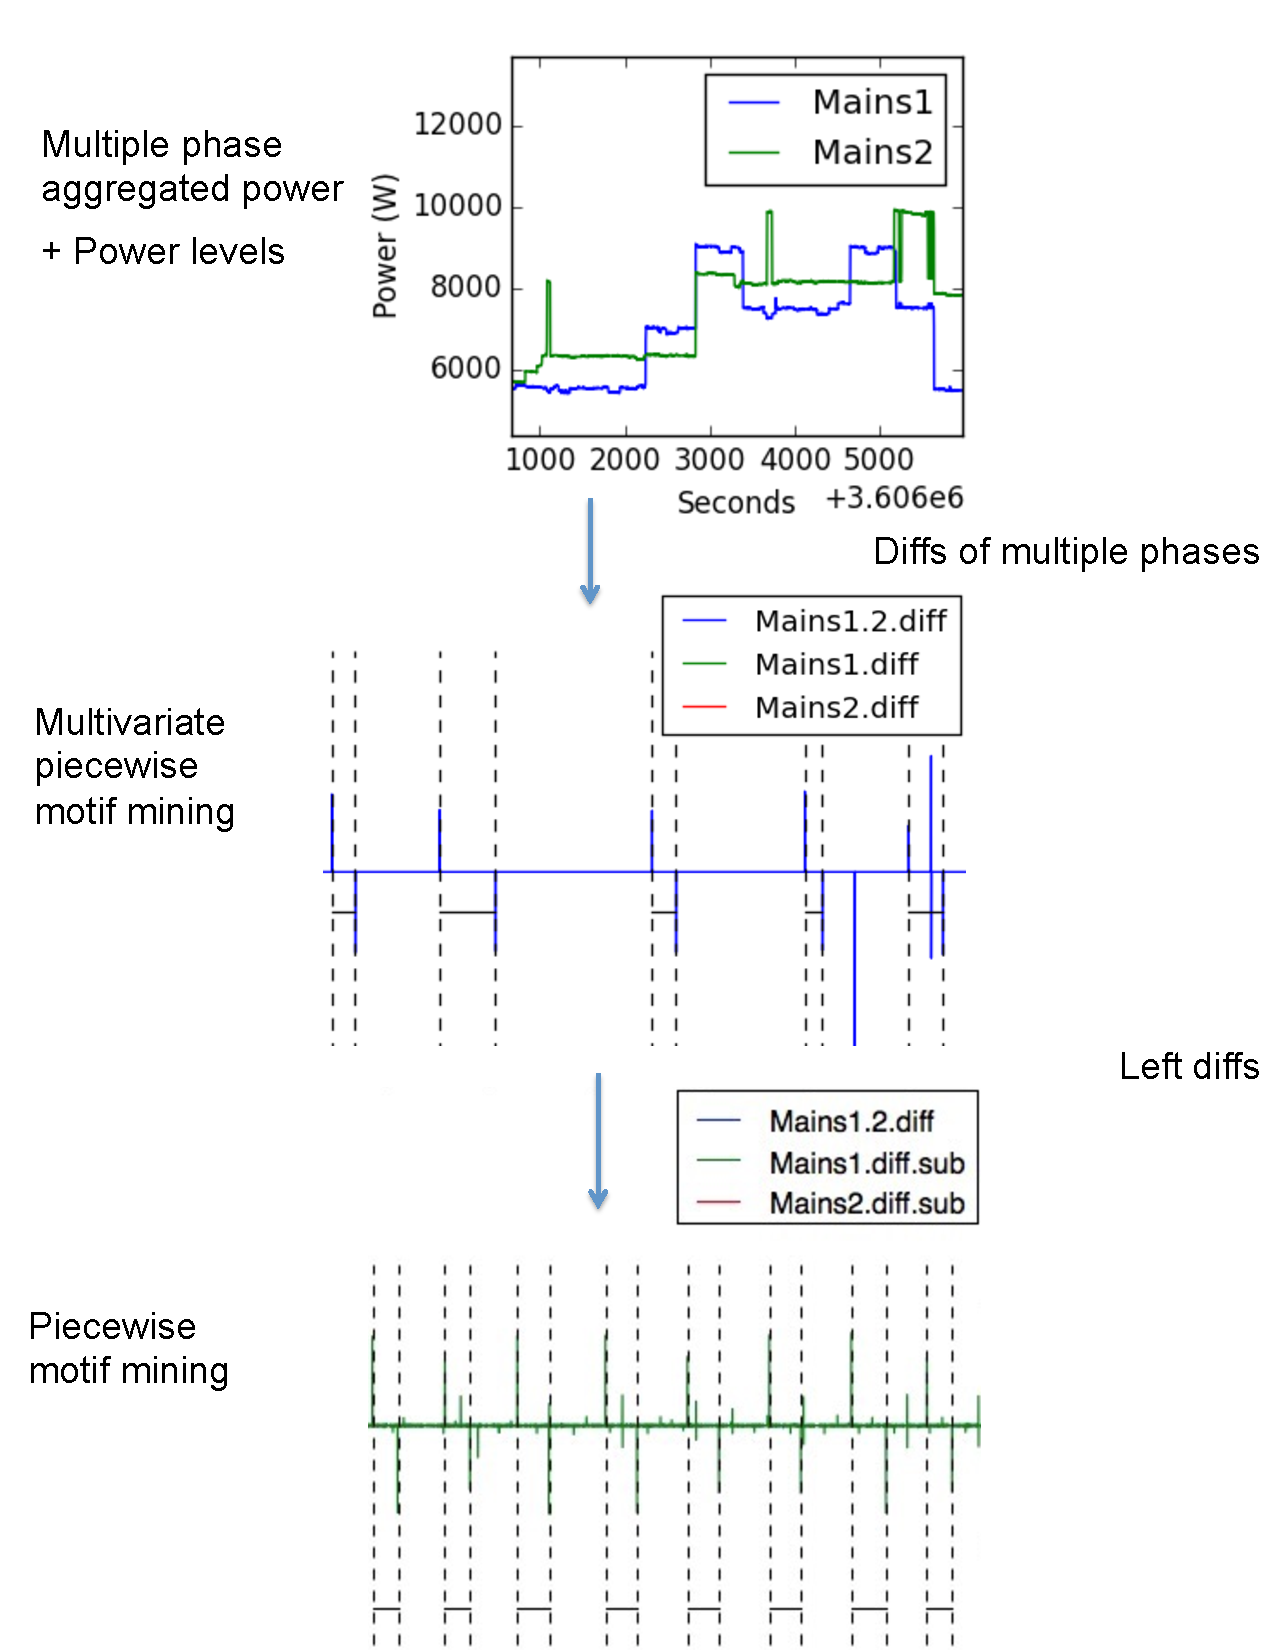
\includegraphics[width=0.5\textwidth]{multidisaggfig/RecursiveMultivariateMotifMining.pdf}
\caption{Recursive Multivariate Motif Mining Approach.}
\label{fig_multivariateMotifming}
\end{figure} 

Generally, multivariate piecewise motif mining is divided into four steps, as shown in Figure \ref{fig_multivariatePiecewiseMotifMining}.
Step 1 is to search for piecewise events from the two-phase or three-phase data.
Step 2 is to encode events from multiple phases. 
Step 3 aims to mine frequent motifs from the encoded events list.
The last step targets to recover devices from mined motifs. 
\begin{figure}[h]
\centering
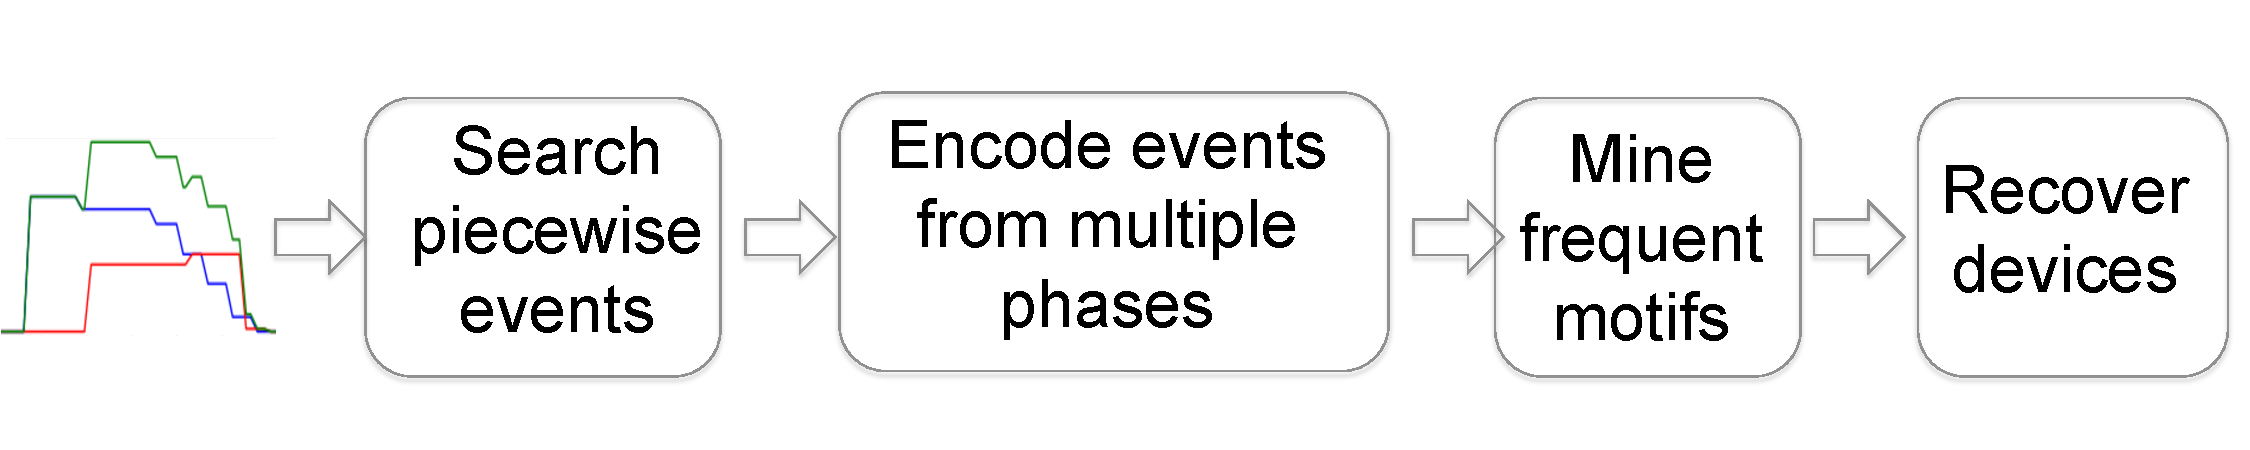
\includegraphics[width=0.5\textwidth]{multidisaggfig/multivariatePiecewiseMotifMining.pdf}
\caption{Multivariate Piecewise Motif Mining.}
\label{fig_multivariatePiecewiseMotifMining}
\end{figure}

\subsection{Piecewise Motif Mining}
Motif mining aims to uncover the repetitive patterns in time series data, and works best for discrete events. Piecewise motif mining is proposed 
for energy disaggregation to detect on/off events. 

\begin{definition}{\textbf{Piecewise Event}}
Given a time series diffs data $y_1, ...., y_{n'}$, where $\forall$ $|y_i| < \eta$. 
A piecewise event is the sum of these $n'$ number of diffs data, $e= \sum_{i=1}^{n'} y_i$. 
\end{definition}
Each piecewise event corresponds to an on/off event of an electric device. 
The value of $\eta$ is the noise range of each device, 
which is usually less than the 10\% of $|e|$.  

\textbf{Piecewise Events Search from Multiple Phases} \\
The majority of electrical devices which draw power from multiple phases consume larger amounts of power than electrical devices which connect to single phase. 
To disaggregate such a device, we need to 
discover specific on/off events features to separate them. 
%on/off events which are yielded by this single device from two-phase or three-phase aggregated data. 
Generally such an electrical device draws power from multiple phases synchronously 
and constructs a  pattern. 
Some devices may consume equal power from both phases all the time,  and so their power consumption patterns from both phases keep the same.
Other devices may show different power usage patterns when drawing power from two phases. 
%The power consumption from both phases may be exactly synchronized and keep the same all the time. 
%Either, the power consumption drawn from a single device differs much. 
\begin{algorithm}
\caption{Search Synchronized Events from Two-phase Aggregated Diffs Data}
\label{alg_synchronizeEvents}
\begin{algorithmic}[1]
\REQUIRE $2$-phases aggregated diffs data $y_k=y_1^{(k)}, ..., y_n^{(k)}$ and $k=1,2$, %each device's power levels and standard deviation $P_m$, $P_m^{std}$, 
big power consumption threshold $\theta$
%\ENSURE $y = x^n$
\FOR{$i=0: n-1$}
\IF { $|y_i^{(1)}| > \theta$}
\FOR{$j=i-5, i+5$}
\IF{ $|y_j^{(1)}| \in [ |y_j^{(2)}| * 0.8, |y_j^{(2)}| *1.2]$}
\STATE $e_i^{(1)}= e_i^{(1)} + y_j^{(1)}$
\STATE $e_i^{(2)}= e_i^{(2)} + y_j^{(2)}$
\ENDIF
\ENDFOR
\STATE $e_i = e_i^{(1)} +e_i^{(2)}$
\ENDIF
\ENDFOR
\RETURN $e_1, ..., e_i, ..., e_{n'}, \forall e_i > 2*\theta$
\end{algorithmic}
\end{algorithm}
Algorithm~\ref{alg_synchronizeEvents} describes how synchronized events from two phases are revealed.  
This input include the two-phase aggregated diffs data and big power consumption threshold $\theta$. 
This threshold guarantees we only discover big power consumption devices. 
We review the phase-1 diffs data. 
If any absolute value $|y_i^{(1)}|$ is greater than $\theta$, 
both previous and posterior five diffs data points from time $i$ are checked. 
For these 10 points values, 
at each time $j$, if the difference between phase-1 $y_i^{(1)}$ and phase-2 $y_i^{(2)}$ is in the range of $0.2*|y_i^{(1)}|$,  
we assert that the diffs data points from these two phases are relatively the same and synchronized. 
The synchronization implies that 
these two identical amounts power consumption comes from a single device. 
Therefore we sum the synchronized power level diffs data and compute the power consumption at time $i$ as $e_i$.  
When $e_i>0$ that denotes an on event, and $e_i<0$ means an off event for a certain device.

Next we transfer these two-phase diffs data into 
an ordered on/off event list $e_1, ..., e_{n'}$,
then we apply motif mining to this events list. 
By matching the devices which consume power greater than $2*\theta$, 
we can separate all devices which draw equal amount of power from two phases.  
%Since we already know the power levels of each device, 
%we just choose those devices which include power levels bigger than $2*\theta$. 
%By applying motif mining, 
%we can separate all devices which consume two-phase power greater than $\theta$ equally. 
%For dataset Study10, we set $\theta=500W$. 
%This approach helps us to discover two devices waterHeater2 and heatingIndoor. 
%All of the on/off events of these two devices are found out. 

\subsection{Encoding Events From Multiple Phases}
After deleting all the synchronized events from phase-1 and phase-2, 
we apply multivariate piecewise motif mining to the remaining phase-1 and phase-2 diffs data, 
to detect devices which consume large amounts of power 
and draw power from two phases synchronously yet unequally. 
There are different power drawing patterns from these two phases.  
We encode these two-phase diffs data, which occur at the same time, as a new event $e$. 
Figure \ref{fig_eventEncoding} gives an example of how the events from two-phase circuits
are encoded. 
We extract an event which consumes power greater than $\theta$, 
then we check five more data points before and after it. 
The values of the 11 data points relevant to this event in Main1.diff are [0, 0, -18, 18, 1093, 1830, -196, -68, -37, -36, 0]. 
The concurrent events listed in Main2.diff are [0, 0, 0, 18, 9, 1946, 440, -51,-36,-36,0]. 
Since the events at the peak occur in the two phases as $(1830, 1946)$, 
and the difference of these two powers $1946-1830=116$ is in the $0.2*1830$ range, 
we consider that these two changes may come from a single device. 
When looking for insight into these two vectors, 
we observe that the sum of the changes of phase 1 is 2604W, and the sum of the changes of phase 2 is 2290W. 
They are in the same range, i.e. $2604*0.8 < 2290$. 
Therefore, we declare that the power changes from these two phases definitely come from a single device. 
We select two of these values and encode them as $e_{1'}=(1093, 9)$, $e_{2'}= (1830, 1946)$
\begin{figure}[h]
\centering
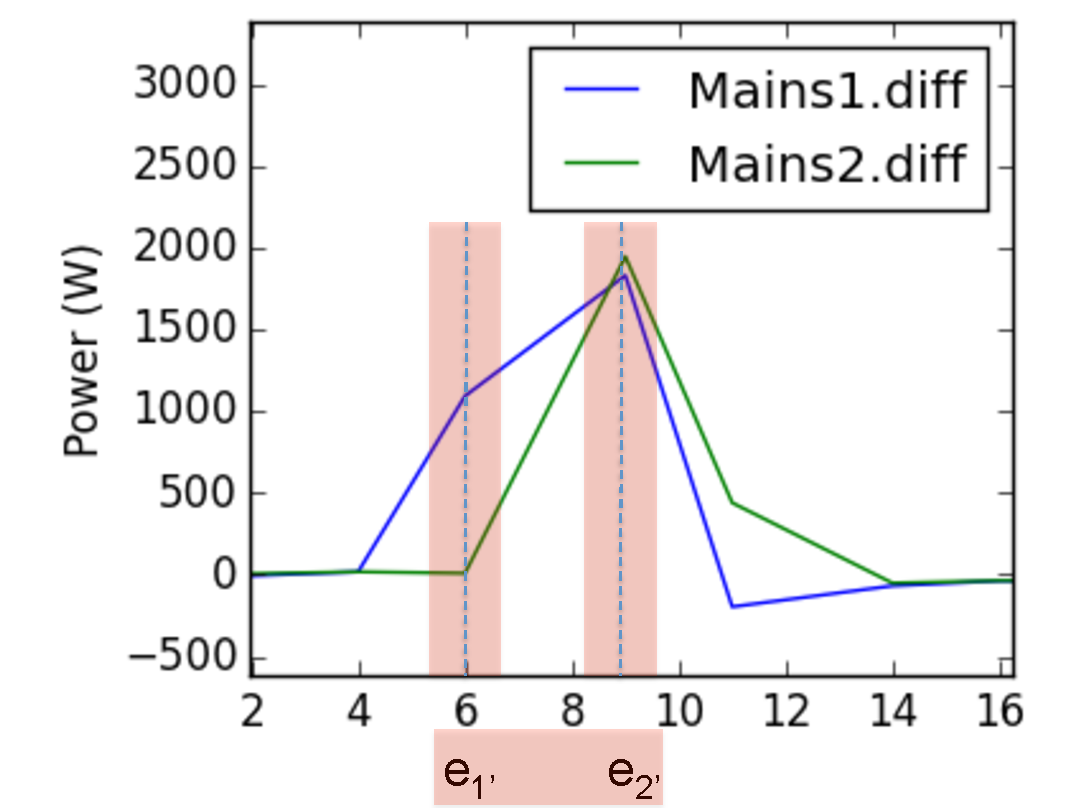
\includegraphics[width=0.3\textwidth]{multidisaggfig/synchronizeDifferentEventEncoding.pdf}
\caption{Encoding Events from Multiple Phases.}
\label{fig_eventEncoding}
\end{figure}

The piecewise events for this single device are $e= [e_{1'}, e_{2'}]$. 
Applying frequent motif mining, 
we separate this large power consumption device which draw power from two phases unequally. 




\section{Evaluation}
%The evaluation tools has been discussed in prior work \cite{liang2010load}.
%
%To evaluate whether each devices is disaggregated or not,
%we need to evaluate two parts, one is how much energy
%is evaluated compared to the ground truth. Another is
%among those disaggregated energy, how much percentage
%are disaggregated right.
%
We use precision, recall and F-measure in our evaluation. The standard
definitions of these metrics are:
%\begin{equation}
$\textrm{precision}=\frac{TP}{TP+FP}$, 
%\end{equation}
%\begin{equation}
$\textrm{recall}=\frac{TP}{TP+FN}$,
%\end{equation}
%\begin{equation}
$\textrm{F-measure}=\frac{1}{\frac{1}{\textrm{precision}}+\frac{1}{\textrm{recall}}}$
%\end{equation}

We need to define the notions of true/false positives
and negatives in the context of disaggregation.

Let us suppose there is a ground truth time series $x$ with length T, 
and denote the corresponding disaggregated time series by $\hat{x}$.
For any time $t \in (0, T)$, there are two values: the
ground truth value of device $m$ is $x_t^{(m)}$ and the disaggregated value
$\hat{x}_t^{(m)}$. We define a parameter $\rho$ for the range of
true values $x_t^{(m)}$, and another parameter $\theta$
as the noise.
For any given measurement, 
there are four total power values or water usage values of device $m$ at
each point: true positive $TP^{(m)}$,  false negative $FN^{(m)}$,
true negative $TN^{(m)}$, and false positive $FP^{(m)}$.

\noindent
1. When $x_t^{(m)} > \theta$ and  $\hat{x}_t^{(m)}> \theta  $,
at this point the disaggregation is a true positive.
There are three situations in turn:

\noindent
1.1. When $  x_t^{(m)} \times (1-\rho) <  \hat{x}_t^{(m)} <  x_t^{(m)} \times (1+\rho)  $, then
\begin{eqnarray*}
 TP^{(m)} &=& \hat{x}_t^{(m)} \\
 FN^{(m)}&=&FP^{(m)} = TN^{(m)}=0
\end{eqnarray*}

\noindent
1.2. When $ \hat{x}_t^{(m)} < x_t^{(m)} \times (1-\rho)$ , then only
the disaggregated power or water usage is considered as true positive and
the power or water usage that is not disaggregated is regarded as a false negative:
\begin{eqnarray*}
TP^{(m)}&=&\hat{x}_t^{(m)} \\
FN^{(m)}&=&x_t^{(m)} - \hat{x}_t^{(m)} \\
FP^{(m)}&=&TN^{(m)}=0
\end{eqnarray*}
1.3 When $ \hat{x}_t^{(m)}>  x_t^{(m)} \times (1+\rho) $, then
the disaggregated power or water usage is a true positive, and those values
which are greater than the truth values are treated as false positive.
\begin{eqnarray*}
TP^{(m)}&=&\hat{x}_t^{(m)} \\
FP^{(m)}&=&\hat{x}_t^{(m)} - x_t^{(m)} \\
FN^{(m)}&=&TN^{(m)}=0
\end{eqnarray*}
2. When $x_t^{(m)} > \theta$ and  $\hat{x}_t^{(m)}< \theta  $,
at this point the disaggregation is a false positive.  Then,
\begin{eqnarray*}
FP^{(m)}&=&x_t^{(m)} \\
TP^{(m)}&=&FN^{(m)} =TN^{(m)}=0
\end{eqnarray*}
3. When $x_t^{(m)} < \theta$ and  $\hat{x}_t^{(m)} > \theta  $,
at this point the disaggregation is a false negative. Then,
\begin{eqnarray*}
FN^{(m)}&=&x_t^{(m)} \\
TP^{(m)}&=&FP^{(m)} = TN^{(m)}=0
\end{eqnarray*}
4. When $x_t^{(m)} < \theta$ and  $\hat{x}_t^{(m)} < \theta  $,
at this point the disaggregation is a true negative.  Then,
\begin{eqnarray*}
TP^{(m)}&=&FN^{(m)} = FP^{(m)} = TN^{(m)}=0
\end{eqnarray*}
%In practice, we use different
%$\rho$ and $\theta$ values depending on the
%dataset. For instance, considering the datasets described below,

In our experimental dataset, we set
$\theta=100$ and $\rho=0.2$. 
Although the maximal power consumption of all these devices is 11000W, 
we can still set $\theta < 11000 * 0.1$ because we apply multivariate piecewise motif mining recursively, 
so the devices which consume a large amount of power are deleted in the first few rounds. 
Therefore the power noise which is caused by the high-power electronic devices 
is greatly decreased. 

\section{Experiments}
We run experiments on the dataset Study10 from the University of Virginia on electricity disaggregation. 
This dataset collects data from 02/10/2014 to 02/21/2014 in a residential building. 
%the following paragraph is from UVa
Two individuals were asked to live in an instrumented home for around two weeks. 
To ensure the data consisted of the personal usage patterns of the participants, 
they were encouraged to live in and use the home as they normally would use their own. 
%The study had institutional review board (IRB) approval and each participant received a \$100 incentive. 
An eMonitor \cite{eMonitor} sensor was used to collect both mains data for testing and circuit-level information for ground truth. 
Additional data, such as the opening of appliance doors and the flicking of light switches, 
was collected to provide sub-circuit level ground truth information for events such as lights.
Both the two-phase aggregated data and each device's data are collected at intervals of 2-3 seconds.
In total, 25 devices were connected to two phases at the entry of the house. 
Five of these devices are seldom operated; less than five times. 
Fourteen devices consume power less than 100W, and the majority of them are lights. 
The largest power consumption of these devices is 11000W by indoor heating. 
The noise caused by the heating device is large; greater than 100W. 
Therefore we focus on disaggregating the six major electronic devices 
with power levels greater than 100W. 
 
% the datasets from University of Virginia on both water and electricity disaggregation. 
%There are totally six data sets. The statistic of these six data set is listed in Table \ref{table_datasets}. 
%The recording interval of these datasets is 2 or 3 seconds. 
%A sensor is instrumented on each device to trace its ground truth operations. 
%\begin{table}[!t]
\renewcommand{\arraystretch}{1.3}
\caption{Electricity Dataset}
\label{table_datasets}
\centering
\begin{tabular}{|c|c|c|c|}
\hline
Data sets & Start date & End date & Duration (day) \\
\hline
\hline
Study 10 & 02-10-2014 & 02-21-2014 & 12\\
\hline
Study 11 & 01-27-2014 & 02-07-2014 & 12\\
\hline
Study 12 & 01-09-2014 & 01-21-2014 & 12\\
\hline
Study 13 & 12-23-2013 & 01-03-2014 & 12\\
\hline
Study 14 & 12-09-2013 & 12-20-2013 & 12\\
\hline
Study 101 & 06-09-2014 & 06-28-2014 & 20\\
\hline
\end{tabular}
\end{table}

\subsection{Electricity Disaggregation}
We assume that we know the power levels of each device. 
If the power levels of each device are unknown, 
we can use the sum of two-phase aggregated data and the on/off events of the 
ground truth to extract them. 
%In order to extract the power level of each device, 
We set a window size $w=30s$ ahead and behind of the ground truth events to match 
the aggregated data.
If there is only one power change in the aggregated data during these 60 seconds, 
this power level change must come from an on/off event of an electrical device. 
Usually, it takes around 2-5 seconds for an electrical device to reach
a steady power level. 
The on and off events reflect different durations for a device to 
reach a steady state. 
Therefore, we measure the minimal duration of the on event and off event 
of each device. 
After we go over all the aggregated data and ground truth on/off events, 
we run a Gaussian mixture model to model the positive power changes and negative power changes
independently. The means and standard deviations correspond to  the on/off event of each device. 
The power levels, standard deviation, and on/off duration of each device of dataset study10 are listed in Table \ref{table_study10results}.
\begin{table*}[!t]
\renewcommand{\arraystretch}{1.3}
\caption{Power Levels, Standard Deviation of Power Levels, On/off Duration, Connected Phases and Disaggregation Results of Electricity Devices from Study10.}
\label{table_study10results}
%\tbl{Power Levels, Standard Deviation of Power Levels, On/off Duration, Connected Phases and Disaggregation Results of Electricity Devices from Study10.\label{table_study10results}}{
\centering
%\small
\footnotesize
%\scriptsize
\setlength\tabcolsep{2pt}
\begin{tabular}{|c|c|c|c|c|c|c|c|c|c|c|}
\hline
\multirow{2}{*}{Device} & Power & Standard & On/off &  \multirow{2}{*}{Phase} & \multicolumn{3}{|c|}{Recursive Multivariate Motif Mining} & \multicolumn{3}{|c|}{AFAMAP}\\
\cline{6-11}
           &  Levels & Deviation & Duration &  &Precision&  Recall &  F-measure & Precision & Recall & F-measure\\ 
\hline
\hline
\multirow{2}{*}{HeatingIndoor+} & \multirow{2}{*}{10590W} & \multirow{2}{*}{1270W} & \multirow{2}{*}{60s} & \multirow{2}{*}{1+2} & \multirow{2}{*}{0.979} & \multirow{2}{*}{0.928} & \multirow{2}{*}{0.953} & \multirow{2}{*}{0.870}& \multirow{2}{*}{0.45} & \multirow{2}{*}{0.598}\\
HeatingOutdoor &  &  &  &  &  &  &  &  & & \\
\hline
Waterheater & 4450W & 350W &  2-5s & 1+2 & 0.999 & 0.997 &0.998 &0.627& 0.882 &0.733\\
\hline
Humidifier & 1470W & 90W & 10s & 1 & 0.997 & 0.992 &0.995 & 0.725 & 0.858 & 0.787\\
\hline
Microwave & 1850W & 200W & 10s & 2 & 0.95 &0.758 & 0.843 & 0.032 & 0.819 & 0.06\\
%\hline
%HeatingOutdoor & 4446W & 140 W & 2-18s & 1+2 &0.308 & 0.66& 0.42& & &\\
\hline
\multirow{2}{*}{Dryer} & 5200W &400W & 2-5s & 1+2 & \multirow{2}{*}{0.911}&\multirow{2}{*}{0.996}&\multirow{2}{*}{0.952}& \multirow{2}{*}{0.011}&\multirow{2}{*}{0.561} & \multirow{2}{*}{0.021}\\
\cline{2-3} \cline{4-5}
                       & 875W &225W  & 2-5s & 1 & & & & & &\\
%\hline
%L007 & 239W & 56W &  2-5s &2 & & & & & &\\
%\hline
%Fridge & 102W & 68W & 2-5s &1& - & - & - & & &\\
%\line
%L010 & 92W & 16W & 2-5s &2& & & & & &\\
%\cline
%L011 & 117W & 29W & 2-5s &1& & & & & &\\
%\hline
%L012 & 104W & 28W & 2-5s & 2& & & & & &\\
\hline
\end{tabular}
%}
\end{table*}


%By analyzing each device, we notice that sometimes the power levels and 
%on/off duration are insufficient to identify the electric devices. 
%For instance, when the device heatingIndoor starts alone, 
%it takes $2-5$ seconds to go to a steady state as shown in Figure \ref{fig_heatingDevices} (a).
%But when the combined device of heatingIndoor and heatingOutdoor 
%starts, the starting duration takes around $4-18$ seconds. 
%In Figure \ref{fig_patterns} (b), after this combined device 
%starts for15 seconds, the power levels changes 
%for 9 times then to a relatively stable state. 
%During this period of 15 seconds, the power changes very rapidly. 
%If we accumulate these power levels together, 
%it's not a fix number. Therefore, for this kind of device, 
%we can only compare the shape of the startup to decide the on events 
%from the aggregated data. 

We apply recursive multivariate piecewise motif mining to dataset Study10 
and compute the precision, recall and F-measure. 
Devices which draw power from both phases are separated first. 
They are heatingIndoor, waterheater and dryer.
\begin{figure*}[!t]
        \centering{
                \begin{tabular}{cc}
                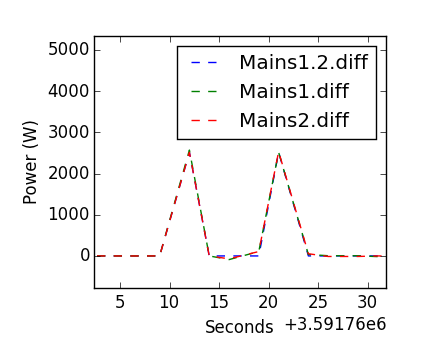
\includegraphics[width=0.5\textwidth]{multidisaggfig/heatingIndoorPhase12On.png} &
                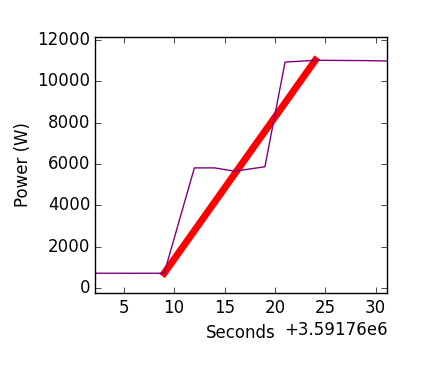
\includegraphics[width=0.5\textwidth]{multidisaggfig/heatingIndoorUp.png}\tabularnewline
                (a) & (b) \tabularnewline
                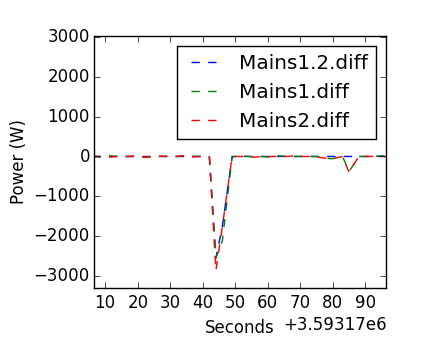
\includegraphics[width=0.5\textwidth]{multidisaggfig/heatingIndoorPhase12Off.png} &
                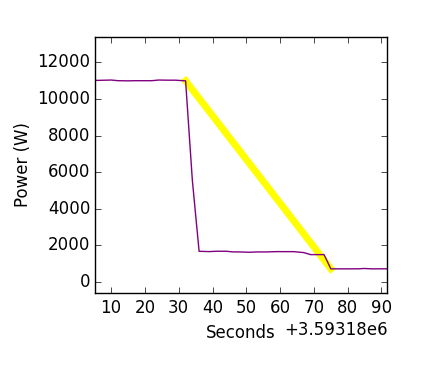
\includegraphics[width=0.5\textwidth]{multidisaggfig/heatingIndoorDown.png}\tabularnewline
                (c) & (d) \tabularnewline
                \end{tabular}
                }
        \caption{
        (a) On piecewise event and (c) Off piecewise event of heatingIndoor. heatingIndoor is disaggregated by motif mining the on event (b) and off event (d).}
        \label{fig_heatingIndoorResults}
\end{figure*}

Figure \ref{fig_heatingIndoorResults} (a) gives an example of 
an on event in the two-phase Mains1 and Mains2. 
Mains1.diff denotes the diffs data from Mains1 and Mains2.diff represents 
the diffs data from Mains2. 
Mains1.2.diff shows as blue when Mains1 and Mains2 share the similar power changes. 
We can see that 
the power consumption of a specific device jumps twice in two phases simultaneously.
The first time, both phases jump 2572W. After nine seconds, 
the power of both phases increases  2520W. 
The sum of these four changes is 10184W. 
Compared with the power levels of all devices, 
we speculate that these power changes are caused 
by the device heatingIndoor. 
%By applying multivariate piecewise motif mining, 
%we match the power consumption with $11000W$ and 
%categorize this on event into heating indoor. 
Figure \ref{fig_heatingIndoorResults} (b) shares the same snippet of time series as Figure \ref{fig_heatingIndoorResults} (a). 
The red line indicates that the on event of heatingIndoor is recognized.    
\begin{figure*}[!t]
        \centering{
                \begin{tabular}{cccc}
                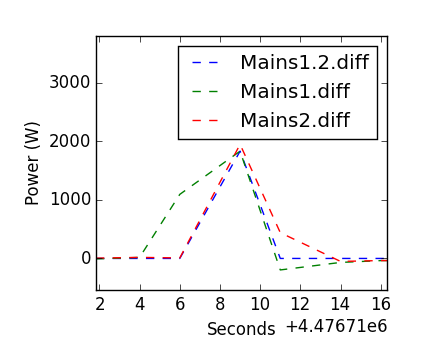
\includegraphics[width=0.5\textwidth]{multidisaggfig/dryerPhase12OnDiff.png} &
                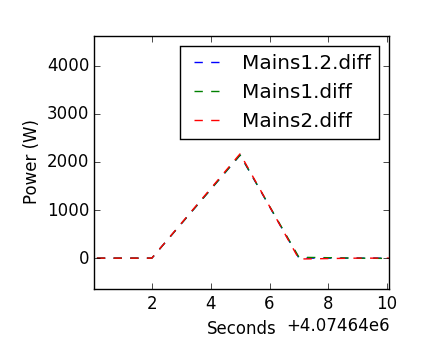
\includegraphics[width=0.5\textwidth]{multidisaggfig/waterHeaterPhase12OnDiff.png} \tabularnewline
                (a) & (b) \tabularnewline
                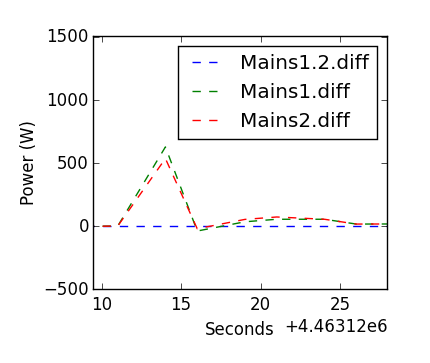
\includegraphics[width=0.5\textwidth]{multidisaggfig/heatingIndoorOutdoorPhase12On_1.png}&
                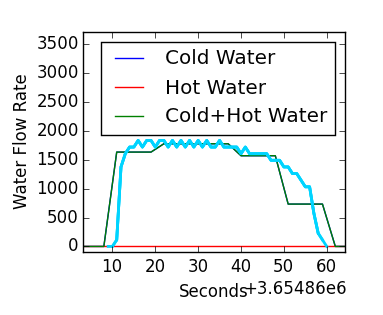
\includegraphics[width=0.5\textwidth]{multidisaggfig/UpToiletFitted.png}\tabularnewline
                (c) & (d) \tabularnewline
                \end{tabular}
                }
        \caption{
        Disaggregating dryer and continuous variable load heatingOutdoor with multivariate motif mining. The on event of a device and the corresponding diffs in the two phases for (a) dryer, (b) water heater, (c) heatingOutdoor. 
  	(d) Disaggregating the toilet water use end with dynamic time-warping subsequence search. This Y-axis is water flow rate in 10000*liter/minute.
        }
        \label{fig_dryerResults}
\end{figure*}

Similarly, the off event plunges twice in two seconds -2877W and -1759W in both phases, as shown in Figure \ref{fig_heatingIndoorResults} (c).
The sum of this off event is -9272W. 
After matching the power levels, we categorize it as the off event of heatingIndoor as indicated in Figure \ref{fig_heatingIndoorResults} (d). 

The dryer has the same power level as the waterheater at around 4800W. 
If we disaggregate these two devices from the sum of the two phases, 
it's difficult to distinguish them,  
but with multivariate piecewise motif mining, these two devices 
can be distinguished. 

%Figure \ref{fig_dryerResults} (a) and (b) shows the on event of dryer from sum of phase 1 and phase 2, 
%and these two phases separately. 
Figure \ref{fig_dryerResults} (a) and (b) are the diff data of the dryer and waterheater from the two-phase circuit. 
We can see that the waterheater draws power from Phase 1 and Phase 2 at the same time,  
but the dryer shows a different pattern. It draws power from Phase 1 at a lower power of 1093W, then jumps to 1830W; 
at the same time, it draws power from Phase 2 at the high level of 1946W immediately. 
We encode the power usage as shown in Figure \ref{fig_eventEncoding}, then apply motif mining to disaggregate them. 
 
After deleting the power consumption from both aggregated phases, 
we apply piecewise motif mining again to a single phase. 
We then discover the humidifier from Phase 1 
and the microwave from Phase 2. 
%Note that the power consumption of humidifier and microwave overlaps sometimes, 
%which makes it hard to separate them. 
%But they draw power from different phases separately. 
%Multivariate motif mining can separate them. 
When we only disaggregate the sum of Phase 1 and Phase 2, 
the precision recall result of the microwave and humidifier is not very accurate 
because sometimes their power consumptions are similar. 
However, using multivariate motif mining, we can separate them very clearly 
with good precision and recall. 
The precision and recall results for the data set Study10 are listed in Table \ref{table_study10results}.

Recursive multivariate motif mining is capable of disaggregating continuous variable loads. 
%\begin{figure*}[!t]
        \centering{
                \begin{tabular}{cccc}
                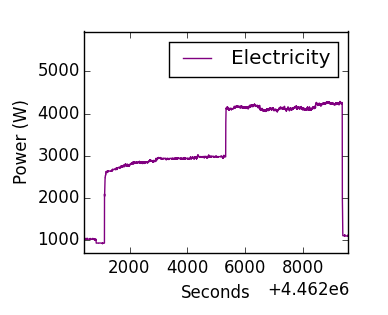
\includegraphics[width=3.2in]{multidisaggfig/heatingIndoorOutdoorPattern1_sum.png} &
                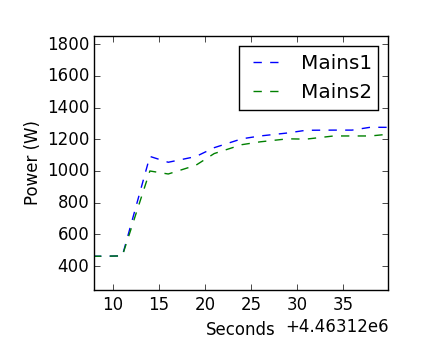
\includegraphics[width=3.2in]{multidisaggfig/heatingIndoorOutdoorPattern1.png} \tabularnewline
                 (a) & (b)\tabularnewline
                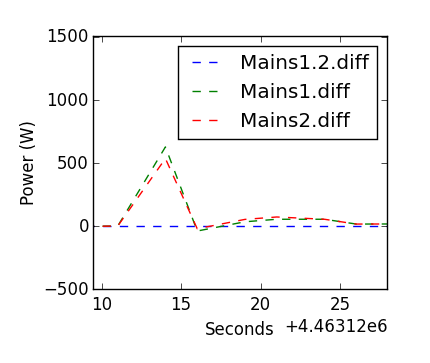
\includegraphics[width=3.2in]{multidisaggfig/heatingIndoorOutdoorPhase12On_1.png} &
                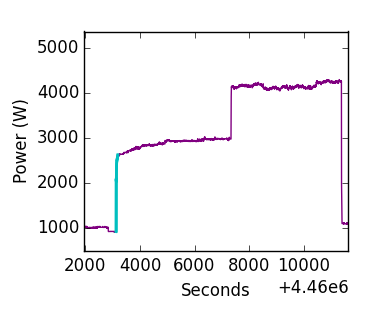
\includegraphics[width=3.2in]{multidisaggfig/heatingIndoorOutdoorFittedPattern1.png}\tabularnewline
                (c) &(d) \tabularnewline
                \end{tabular}
                }
        \caption{
        Disaggregating continuous variable load heating outdoor. 
        (a) the startup in the sum of aggregated power (b) the startup in two phases (c) the diffs in two phases (d) the disaggregated on event of heating outdoor.}
        \label{fig_heatingOutdoorResults}
\end{figure*}

Figure \ref{fig_dryerResults} (c) shows the diff data of heatingOutdoor from the two phases. 
During this on event, its power levels change nine times, then continue at a relatively stable state.
%Figure \ref{fig_heatingOutdoorResults} (a) illustrates the startup of heatingOutdoor.
%as shown in Figure \ref{fig_heatingOutdoorResults} (b) and (c). 
By applying piecewise motif mining, 
we can successfully identify this as the heatingOutdoor device 
after matching its power level. 
%The disaggregated result is displayed in Figure \ref{fig_dryerResults} (d).
%Note that this continuous variable load startup snippet can be discovered by dynamic time warping 
%subsequence search as well if this device is on without the intervene of other devices.
If another device  $D$ which draws from Phase 1 or Phase 2 is turned on or off during this period, 
multivariate piece-wise motif mining can still identify this heatingOutdoor device. 
This is because $D$ only uses one phase's power; 
hence its power change is not counted in our piecewise event. 

\subsection{Water Disaggregation and Constraints}
Water usage displays different characteristics. 
The total water consumption is zero most of the time.
Whenever a water use end is operated, water is consumed intensively for a period of time. 
Then it will stay off for a much longer time. 
We observe that the operations of water use ends reflect a series of user behaviors. 
For instance, a person may use the toilet in the bathroom first, 
then wash hands in the sink and finally take a shower afterwards. 
%This series of events highly affect electricity usage as well. 
%When the person enters into the bathroom, the light in the bathroom is turned on. 
%After using the bathroom, the person leaves and turns the light off. 
%Moreover, we observe that the usage of toilet is usually accompanied by
%sink usage afterwards. 

%In this subsection, we apply the semi-supervised multivariate piecewise motif mining 
%to water data. 
Similar to electricity disaggregation, we use a period of aggregated water usage 
data to extract features  
and obtain the water flow rate level of each water use end.
Table \ref{table_resultStudy10Water} lists the water consumption rate for each device. 
For instance, taking a shower uses hot water at a flow rate between 0.1822 liter/min and 0.1986 liter/min. 
Let $\frac{\alpha}{10000}$ denotes this range of water flow rate.
The total hot and cold water consumption by  shower is 0.1904 liter/min. 
Therefore, the cold water flow rate caused by shower is $0.1904-\frac{\alpha}{10000}$ liter/min. 
Turning on the water for the shower takes around two seconds. 
%The disaggregation results are shown in Table \ref{table_resultStudy10Water}.
%\begin{table*}[!t]
\renewcommand{\arraystretch}{1.3}
%\caption{Water Flow Rate Levels of Water End Uses and Disaggregation Results}
%\label{table_resultStudy10Water}
\tbl{Water Flow Rate Levels of Water End Uses and Disaggregation Results.\label{table_resultStudy10Water}}{
\centering
\begin{tabular}{|c|c|c|c|c|c|c|}
\hline
\multirow{2}{*}{Device} & \multirow{2}{*}{Hot water} & \multirow{2}{*}{Cold water} & \multirow{2}{*}{Duration} &  \multirow{2}{*}{Precision} & \multirow{2}{*}{Recall} &  \multirow{2}{*}{F-measure}\\
           &  (liter/min) & (l/min*10000)& (second) & & & \\
\hline
\hline
Shower & $\alpha \in (1822, 1986)$ & $1904-\alpha$& on: 2 & 0.999 & 0.972 & 0.986 \\
\hline
Washing Machine & $\alpha \in (1988, 2276)$  & $2132-\alpha$ & on: 5& 0.997  & 0.969 & 0.983\\
\hline
DownToilet & 0 & (1270, 1400) & whole: 50& NA & NA & NA\\
\hline
UpToilet & 0 & (1480, 1700) & whole: 50& NA & NA & NA \\
%\hline
%KitchenSink &  $ \alpha \in (0, 57) $ & 57- $\alpha$ & 2& & & \\
%\hline
%UpSink & 34 & 160 & 2& & & \\
%\hline
%DownSink & 57  & 80 & 2& & & \\
%\hline
%Dish Washer & 34 & -11 & 2& & & \\
\hline
\end{tabular}
}
\end{table*}
\begin{table}[h]
\renewcommand{\arraystretch}{1.3}
\caption{Water Flow Rate Levels of Water End Uses.}
\label{table_resultStudy10Water}
\centering
\small
\setlength\tabcolsep{2pt}
\begin{tabular}{|c|c|c|c|c|c|c|}
\hline
\multirow{2}{*}{Device} & \multirow{2}{*}{Hot water} & \multirow{2}{*}{Cold water} & \multirow{2}{*}{Duration}  \\
           &  (liter/min*10000) & (l/min*10000)  & (second)\\
\hline
\hline
Shower & $\alpha \in (1822, 1986)$ & $1904-\alpha$  & on: 2\\
\hline
Washing Machine & $\alpha \in (1988, 2276)$  & $2132-\alpha$ & on: 5\\
\hline
DownToilet & 0 & (1270, 1400) & whole: 50\\
\hline
UpToilet & 0 & (1480, 1700) & whole: 50\\
%\hline
%KitchenSink &  $ \alpha \in (0, 57) $ & 57- $\alpha$ & 2& & & \\
%\hline
%UpSink & 34 & 160 & 2& & & \\
%\hline
%DownSink & 57  & 80 & 2& & & \\
%\hline
%Dish Washer & 34 & -11 & 2& & & \\
\hline
\end{tabular}
\end{table}

After these calculations, we apply a multivariate piecewise motif mining approach to 
water disaggregation. 
For the shower and washing machine, 
the total flow rate of hot and cold water is high,  nearly 0.2 liter/minute. 
Therefore by only searching the 
total hot and cold water flow rate, we can identify these two devices. 
The event of shower usage usually lasts for more than one minute, 
but the washing machine uses water for less than one minute, 
repeating six to nine times. 
Both the shower and washing machine use 
hot water and cold water. 
However, the washing machine uses hot water for only the 
first one or two times. For the rest of its cycle, 
only cold water is used. 
Whenever the washing machines starts, 
the power consumption starts as well. 

%\begin{figure*}[!t]
        \centering{
                \begin{tabular}{cc}
                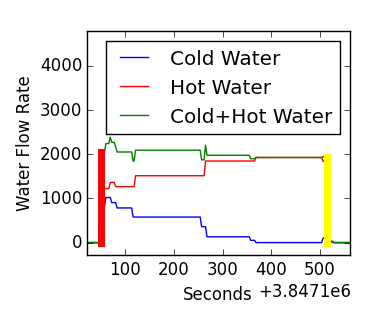
\includegraphics[width=0.5\textwidth]{multidisaggfig/showerFitted.png}&
                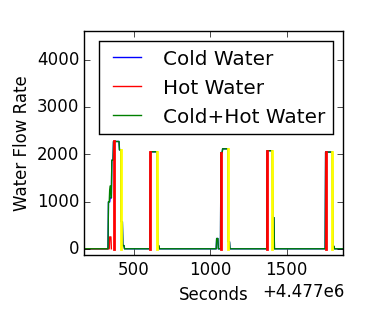
\includegraphics[width=0.5\textwidth]{multidisaggfig/washingMachineWaterFitted.png}\tabularnewline
                (a) & (b)\tabularnewline
                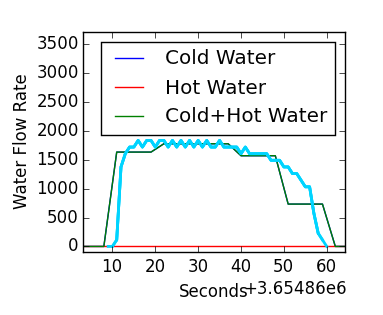
\includegraphics[width=0.5\textwidth]{multidisaggfig/UpToiletFitted.png}&
                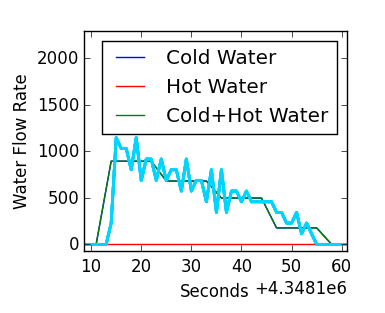
\includegraphics[width=0.5\textwidth]{multidisaggfig/DownToiletFitted.png}
                \tabularnewline
                 (c) & (d)\tabularnewline
                \end{tabular}
                }
        \caption{
        X-axis is the duration to a specific time in seconds, Y-axis is water flow rate in 10000*liter/minute. 
	(a) and (b) denote the water disaggregation of shower and washing machine. The fitted red line denotes the on event of water, and the fitted yellow line denotes the off event of water. 
	(c) and (d) are the disaggregated two toilets of complete usage cycle by dynamic time warping subsequence search. 
	}
        \label{fig_waterDisaggResults}
\end{figure*}
%Figure \ref{fig_waterDisaggResults} (a) and (b) display the water usage of shower and washing machine. 
Applying piecewise motif mining to the water usage lets us disaggregate the
shower and washing machine. %as in Figure \ref{fig_waterDisaggResults} (a) and (b).
The precision, recall and F-measure for the shower disaggregation are 
0.999, 0.972, and 0.986,  
and the precision, recall and F-measure for the washing machine disaggregation are 
0.997, 0.969, and 0.983. 
However, with a variable water flow rate, 
piecewise motif mining has limitations in handling water use ends such as the toilet.
Therefore we use the dynamic time warping subsequence~\cite{rakthanmanon2012searching} search as a complementary to discover these water use ends.  
For the two toilets, we apply dynamic time warping to match the time series.
The water usage results of one toilet, UpToilet, is shown in Figure \ref{fig_dryerResults} (d). 

%There are totally three sinks in the house, namely up sink, down sink and kitchen sink. 
%People may use sinks with only hot water or cold water, or both hot and cold water. 
%The water usage may be large or small. 
%In this case, it is hard to distinguish these three sinks. 
%However, by observing the water usage of up sink and down sink. 
%We find that there's correlation between the down sink and the down toilet, 
%up sink and up toilet. 
%Figure \ref{fig_ToiletSinkCorrelation} (a) and (b) show that the toilet and sink start almost at the same time, 
%or end at the same time. 
We can see that multivariate piecewise motif mining is capable of 
disaggregating water use ends which have sharp on/off water flow rates. 
However, it has limitations in dealing with water use ends with irregular water use patterns, 
such as toilets and sinks. 
Since the water usage of toilets is relatively fixed if used alone, 
some toilet water usages can be disaggregated by using the dynamic time warping subsequence search 
which was researched in \cite{nguyen2013development}. 


%\subsection{Electricity and Water Usage Correlation}
%From the above electricity and water disaggregation, 
%we observe that some devices, such as washing machine, use both electricity and water. 
%We extend our multivariate episode mining approach 
%from disaggregating two time series of hot water and cold water, 
%to three time series of hot water, cold water and electricity. 

We discover that water usage is more like a series of human behavior, as in Figure \ref{fig_bathroomBehavior}.
One person turns on the light L007 in the bathroom,  uses the toilet, flushes and wash hands,
accompanied by  taking  a shower and leaving the bathroom with the light turned off. 
\begin{figure}[!t]
\centering
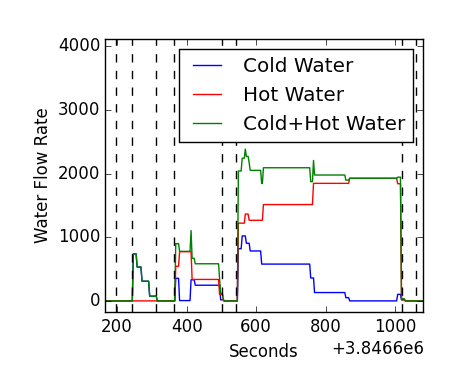
\includegraphics[width=0.7\textwidth]{multidisaggfig/bathroomBehavior.png}
\caption{Human behavior in bathroom by using down toilet, down sink and shower. The dashed lines denote 
a series of events: light L007 on, down toilet on,  down toilet off, down sink on, down sink off, shower on, shower off, light L007 off. }
\label{fig_bathroomBehavior}
\end{figure}

\begin{comment}
\begin{table}[!t]
\renewcommand{\arraystretch}{1.3}
\caption{Washing Machine Disaggregation with Multivariate Episode Mining}
\label{table_washingMachineDisagg}
\centering
\begin{tabular}{|c|c|c|c|c|}
\hline
Aggregated Data & Disaggregation Type& Precision  & Recall & F-Measure\\
\hline
\hline
Electricity & Single & 0.8 & 0.9 & 0.88\\
\hline
Water & Multivariate& 0.8 & 0.9 & 0.88\\
\hline
Electricity and Water & Multivariate & 0.8 & 0.9 & 0.88\\
\hline
\end{tabular}
\end{table}
\end{comment}
\section{Conclusion}
This paper proposes a semi-supervised recursive multivariate piecewise motif mining approach 
to electricity disaggregation. 
%Before unsupervised disaggregation, 
We use data from a period of time to find the features of individual devices, 
including the power level and standard deviation.
Based on these features, 
we recursively utilize multivariate motif mining to uncover devices 
that draw power from both phases equally or unequally, 
then separate the devices from each phase using motif mining. 
Devices that use a large amount of power are removed from the two phases in the first few rounds, 
which brings the benefit of decreasing the noise caused by these devices 
during the process of disaggregating from single phase. 
Therefore more devices with smaller power consumption are separated 
using the piecewise motif mining from a single phase. 
In addition, this piecewise motif mining approach can identify
continuously variable loads such as outdoor heating. 
Furthermore, when we apply motif mining approach to water disaggregation, 
it can separate water use ends that have steady water usage, such as a shower, 
but cannot disaggregate those water use ends which consume water variably for the whole 
cycle, like a toilet. 

In the future, 
for energy disaggregation we will use more features from the aggregated data from the multiple phases, 
such as the startup shape of individual devices.
For water disaggregation, we will explore how to integrate the 
dynamic time warping with multivariate piecewise motif mining. 
 

\bibliographystyle{ACM-Reference-Format}
\bibliography{references} 

\end{document}
